% xcolor and define colors -------------------------
\usepackage{xcolor}

% https://www.viget.com/articles/color-contrast/
\definecolor{purple}{HTML}{5601A4}
\definecolor{navy}{HTML}{0D3D56}
\definecolor{ruby}{HTML}{9a2515}
\definecolor{alice}{HTML}{107895}
\definecolor{daisy}{HTML}{EBC944}
\definecolor{coral}{HTML}{F26D21}
\definecolor{kelly}{HTML}{829356}
\definecolor{cranberry}{HTML}{E64173}
\definecolor{jet}{HTML}{131516}
\definecolor{asher}{HTML}{555F61}
\definecolor{slate}{HTML}{314F4F}

% Mixtape Sessions
\definecolor{picton-blue}{HTML}{00b7ff}
\definecolor{violet-red}{HTML}{ff3881}
\definecolor{sun}{HTML}{ffaf18}
\definecolor{electric-violet}{HTML}{871EFF}

\newcommand\pictonBlue[1]{{\color{picton-blue}#1}}
\newcommand\sun[1]{{\color{sun}#1}}
\newcommand\electricViolet[1]{{\color{electric-violet}#1}}
\newcommand\violetRed[1]{{\color{violet-red}#1}}

\newcommand\bgPictonBlue[1]{{\colorbox{picton-blue!20!white}{#1}}}
\newcommand\bgSun[1]{{\colorbox{sun!20!white}{#1}}}
\newcommand\bgElectricViolet[1]{{\colorbox{electric-violet!20!white}{#1}}}
\newcommand\bgVioletRed[1]{{\colorbox{violet-red!20!white}{#1}}}

\def\code#1{\texttt{#1}}

% Main theme colors
\definecolor{accent}{HTML}{00b7ff}
\definecolor{accent2}{HTML}{871EFF}
\definecolor{gray100}{HTML}{f3f4f6}
\definecolor{gray800}{HTML}{1F292D}


% Beamer Options -------------------------------------

% Background
\setbeamercolor{background canvas}{bg = white}

% Change text margins
\setbeamersize{text margin left = 15pt, text margin right = 15pt} 

% \alert
\setbeamercolor{alerted text}{fg = accent2}

% Frame title
\setbeamercolor{frametitle}{bg = white, fg = jet}
\setbeamercolor{framesubtitle}{bg = white, fg = accent}
\setbeamerfont{framesubtitle}{size = \small, shape = \itshape}

% Block
\setbeamercolor{block title}{fg = white, bg = accent2}
\setbeamercolor{block body}{fg = gray800, bg = gray100}

% Title page
\setbeamercolor{title}{fg = gray800}
\setbeamercolor{subtitle}{fg = accent}

%% Custom \maketitle and \titlepage
\setbeamertemplate{title page}
{
    %\begin{centering}
        \vspace{20mm}
        {\Large \usebeamerfont{title}\usebeamercolor[fg]{title}\inserttitle}\\
        {\large \itshape \usebeamerfont{subtitle}\usebeamercolor[fg]{subtitle}\insertsubtitle}\\ \vspace{10mm}
        {\insertauthor}\\
        {\color{asher}\small{\insertdate}}\\
    %\end{centering}
}

% Table of Contents
\setbeamercolor{section in toc}{fg = accent!70!jet}
\setbeamercolor{subsection in toc}{fg = jet}

% Button 
\setbeamercolor{button}{bg = accent}

% Remove navigation symbols
\setbeamertemplate{navigation symbols}{}

% Table and Figure captions
\setbeamercolor{caption}{fg=jet!70!white}
\setbeamercolor{caption name}{fg=jet}
\setbeamerfont{caption name}{shape = \itshape}

% Bullet points

%% Fix spacing between items
\let\olditemize=\itemize 
\let\endolditemize=\enditemize 
\renewenvironment{itemize}{\vspace{0.25em}\olditemize \itemsep0.25em}{\endolditemize}

%% Fix left-margins
\settowidth{\leftmargini}{\usebeamertemplate{itemize item}}
\addtolength{\leftmargini}{\labelsep}

%% enumerate item color
\setbeamercolor{enumerate item}{fg = accent}
\setbeamerfont{enumerate item}{size = \small}
\setbeamertemplate{enumerate item}{\insertenumlabel.}

%% itemize
\setbeamercolor{itemize item}{fg = accent!70!white}
\setbeamerfont{itemize item}{size = \small}
\setbeamertemplate{itemize item}[circle]

%% right arrow for subitems
\setbeamercolor{itemize subitem}{fg = accent!60!white}
\setbeamerfont{itemize subitem}{size = \small}
\setbeamertemplate{itemize subitem}{$\rightarrow$}

\setbeamertemplate{itemize subsubitem}[square]
\setbeamercolor{itemize subsubitem}{fg = jet}
\setbeamerfont{itemize subsubitem}{size = \small}








% Links ----------------------------------------------

\usepackage{hyperref}
\hypersetup{
  colorlinks = true,
  linkcolor = accent2,
  filecolor = accent2,
  urlcolor = accent2,
  citecolor = accent2,
}


% Line spacing --------------------------------------
\usepackage{setspace}
\setstretch{1.35}


% \begin{columns} -----------------------------------
\usepackage{multicol}


% Fonts ---------------------------------------------
% Beamer Option to use custom fonts
\usefonttheme{professionalfonts}

% \usepackage[utopia, smallerops, varg]{newtxmath}
% \usepackage{utopia}
\usepackage[sfdefault,light]{roboto}

% Small adjustments to text kerning
\usepackage{microtype}



% Remove annoying over-full box warnings -----------
\vfuzz2pt 
\hfuzz2pt


% Table of Contents with Sections
\setbeamerfont{myTOC}{series=\bfseries, size=\Large}
\AtBeginSection[]{
        \frame{
            \frametitle{Roadmap}
            \tableofcontents[current]   
        }
    }


% Tables -------------------------------------------
% Tables too big
% \begin{adjustbox}{width = 1.2\textwidth, center}
\usepackage{adjustbox}
\usepackage{array}
\usepackage{threeparttable, booktabs, adjustbox}
    
% Fix \input with tables
% \input fails when \\ is at end of external .tex file
\makeatletter
\let\input\@@input
\makeatother

% Tables too narrow
% \begin{tabularx}{\linewidth}{cols}
% col-types: X - center, L - left, R -right
% Relative scale: >{\hsize=.8\hsize}X/L/R
\usepackage{tabularx}
\newcolumntype{L}{>{\raggedright\arraybackslash}X}
\newcolumntype{R}{>{\raggedleft\arraybackslash}X}
\newcolumntype{C}{>{\centering\arraybackslash}X}

% Figures

% \imageframe{img_name} -----------------------------
% from https://github.com/mattjetwell/cousteau
\newcommand{\imageframe}[1]{%
    \begin{frame}[plain]
        \begin{tikzpicture}[remember picture, overlay]
            \node[at = (current page.center), xshift = 0cm] (cover) {%
                \includegraphics[keepaspectratio, width=\paperwidth, height=\paperheight]{#1}
            };
        \end{tikzpicture}
    \end{frame}%
}

% subfigures
\usepackage{subfigure}


% Highlight slide -----------------------------------
% \begin{transitionframe} Text \end{transitionframe}
% from paulgp's beamer tips
\newenvironment{transitionframe}{
    \setbeamercolor{background canvas}{bg=accent!40!black}
    \begin{frame}\color{accent!10!white}\LARGE\centering
}{
    \end{frame}
}


% Table Highlighting --------------------------------
% Create top-left and bottom-right markets in tabular cells with a unique matching id and these commands will outline those cells
\usepackage[beamer,customcolors]{hf-tikz}
\usetikzlibrary{calc}
\usetikzlibrary{fit,shapes.misc}

% To set the hypothesis highlighting boxes red.
\newcommand\marktopleft[1]{%
    \tikz[overlay,remember picture] 
        \node (marker-#1-a) at (0,1.5ex) {};%
}
\newcommand\markbottomright[1]{%
    \tikz[overlay,remember picture] 
        \node (marker-#1-b) at (0,0) {};%
    \tikz[accent!80!jet, ultra thick, overlay, remember picture, inner sep=4pt]
        \node[draw, rectangle, fit=(marker-#1-a.center) (marker-#1-b.center)] {};%
}


% DAGS ----------------------------------------------
\usepackage{tikz}
\usetikzlibrary{shapes,decorations,arrows,calc,arrows.meta,fit,positioning}
% Tikz settings optimized for causal graphs.
\tikzset{
    -Latex,auto,node distance =1 cm and 1 cm,semithick,
    state/.style ={ellipse, draw, minimum width = 0.7 cm},
    point/.style = {circle, draw, inner sep=0.04cm,fill,node contents={}},
    bidirected/.style={Latex-Latex,dashed},
    el/.style = {inner sep=2pt, align=left, sloped}
}


% Beamer tricks -------------------------------------
% Make \pause work in align environments
\makeatletter
\renewrobustcmd{\beamer@@pause}[1][]{%
  \unless\ifmeasuring@%
  \ifblank{#1}%
    {\stepcounter{beamerpauses}}%
    {\setcounter{beamerpauses}{#1}}%
  \onslide<\value{beamerpauses}->\relax%
  \fi%
}
\makeatother


\title [Bootstrap]{ Cross Validation and Sample Splitting}
\author{C.Conlon}
\institute{Applied Econometrics II}
\date{\today}
\setbeamerfont{equation}{size=\tiny}
\begin{document}

\begin{frame}
\titlepage
\end{frame}



\begin{frame}{Cross Validation}
Cross Validation appears superficially similar to bootstrap but asks a different question.
\begin{itemize}
\item Bootstrap tries to construct an empirical analogue to the sampling distribution of $\hat{\theta}$.
\item CV tries to measure what the expected out of sample (OOS or EPE) prediction error of a new never seen before dataset.
\item The main consideration is to prevent \alert{overfitting}.
\begin{itemize}
\item In sample fit is always going to be maximized by the most complicated model.
\item OOS fit might be a different story.
\item 1-NN might do really well in-sample, but with a new sample might perform badly.
\end{itemize}
\end{itemize}
\end{frame}

\begin{frame}{Sample Splitting/Holdout Method and CV}
Cross Validation is actually a more complicated version of \alert{sample splitting} that is one of the organizing principles in machine learning literature.

\begin{description}
\item[Training Set] This is where you estimate parameter values.
\item[Validation Set] This is where you choose a model- a bandwidth $h$ or tuning parameter $\lambda$ by computing the error.
\item[Test Set] You are only allowed to look at this after you have chosen a model. \alert{Only Test Once}: compute the error again on fresh data.
\end{description}
\begin{itemize}
\item Conventional approach is to allocate 50-80\% to training and 10-20\% to Validation and Test.
\item Sometimes we don't have enough data to do this reliably.
\end{itemize}
\end{frame}

\begin{frame}{Sample Splitting/Holdout Method}
\begin{center}
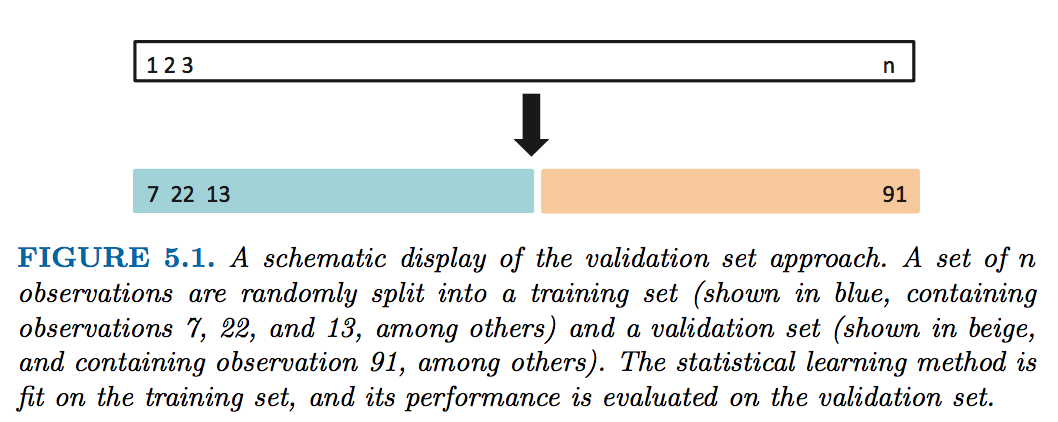
\includegraphics[width=4.5in]{./resources/split-sample}
\end{center}
\end{frame}

\begin{frame}{Challenge with Sample Splitting}
\begin{center}
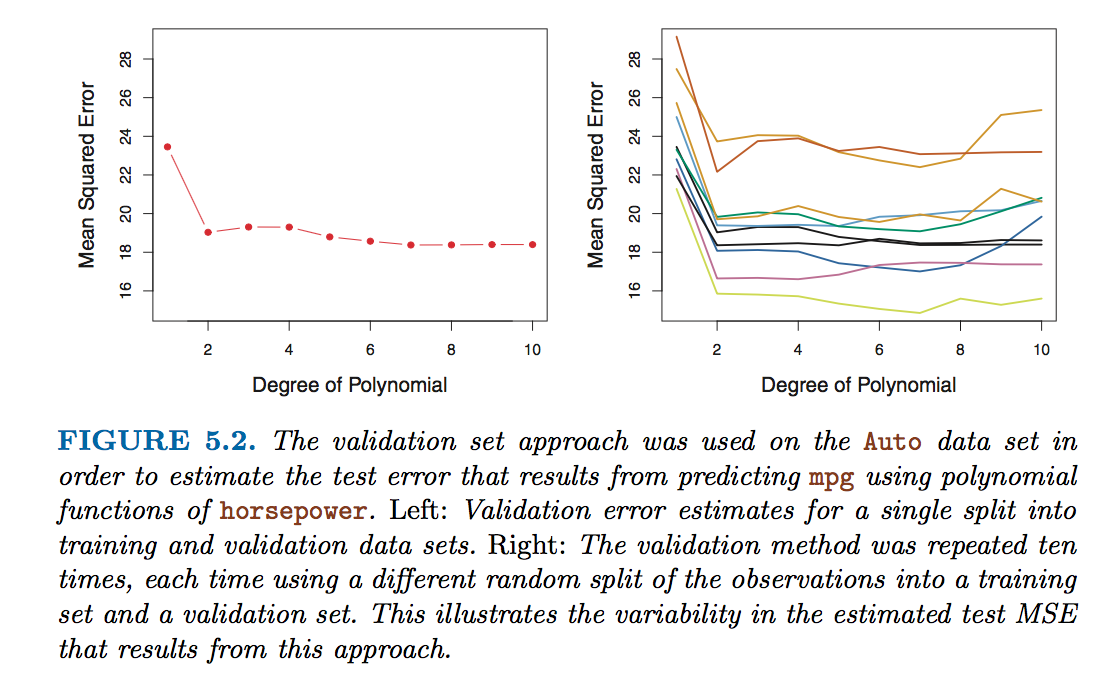
\includegraphics[width=4.5in]{./resources/validation-10fold}
\end{center}
\end{frame}


\begin{frame}{Cross Validation}
\begin{center}
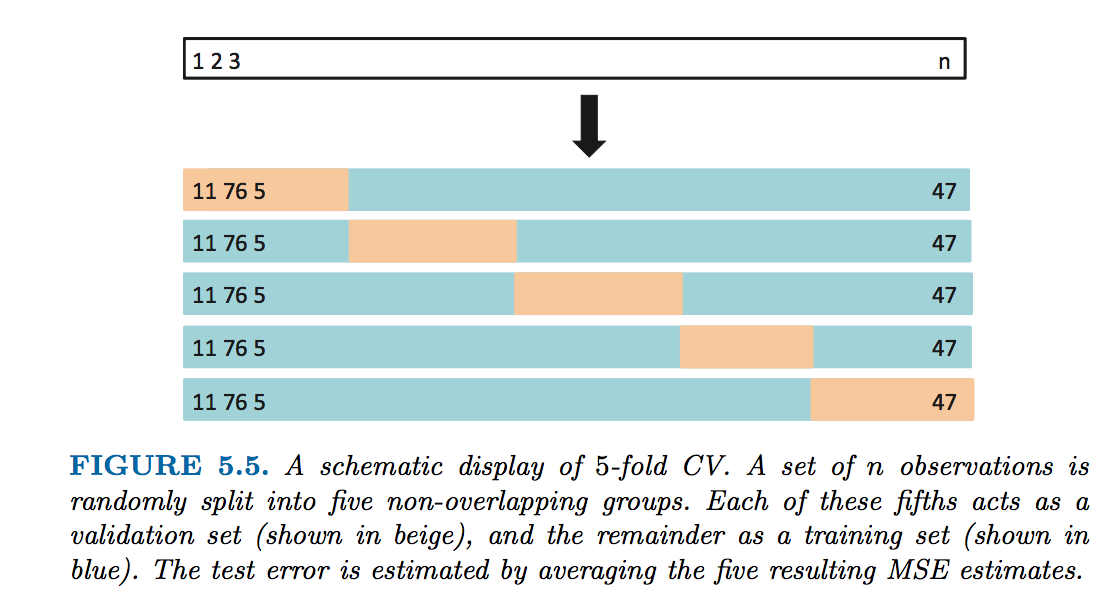
\includegraphics[width=4.5in]{./resources/split-cv5}
\end{center}
\end{frame}

\begin{frame}{$k$-fold Cross Validation}
\begin{itemize}
\item Break the dataset into $k$ equally sized ``folds'' (at random).
\item Withhold $i=1$ fold
\begin{itemize}
\item Estimate the model parameters $\hat{\theta}^{(-i)}$ on the remaining $k-1$ folds
\item Predict $\hat{y}^{(-i)}$ using $\hat{\theta}^{(-i)}$ estimates for the $i$th fold (withheld data).
\item Compute $MSE_i =\frac{1}{k \cdot N} \sum_j (y^{(-i)}_j -\hat{y}^{(-i)}_j)^2$.
\item Repeat for $i=1,\ldots,k$.
\end{itemize}
\item Construct $\widehat{MSE}_{k,CV} = \frac{1}{k} \sum_i MSE_{i}$
\end{itemize}
\end{frame}

\begin{frame}{Leave One Out Cross Validation (LOOCV)}
Same as $k$-fold but with $k=N$.
\begin{itemize}
\item Withhold a single observation $i$
\item Estimate $\hat{\theta}_{(-i)}$.
\item Predict $\hat{y}_i$ using $\hat{\theta}^{(-i)}$ estimates
\item Compute $MSE_i =\frac{1}{N} \sum_j (y_i -\hat{y}_i(\hat{\theta}^{(-i)}))^2$.
\end{itemize}
\vspace{0.2cm}
Note: this requires estimating the model $N$ times which can be costly.
\end{frame}



\begin{frame}{Cross Validation}
\begin{center}
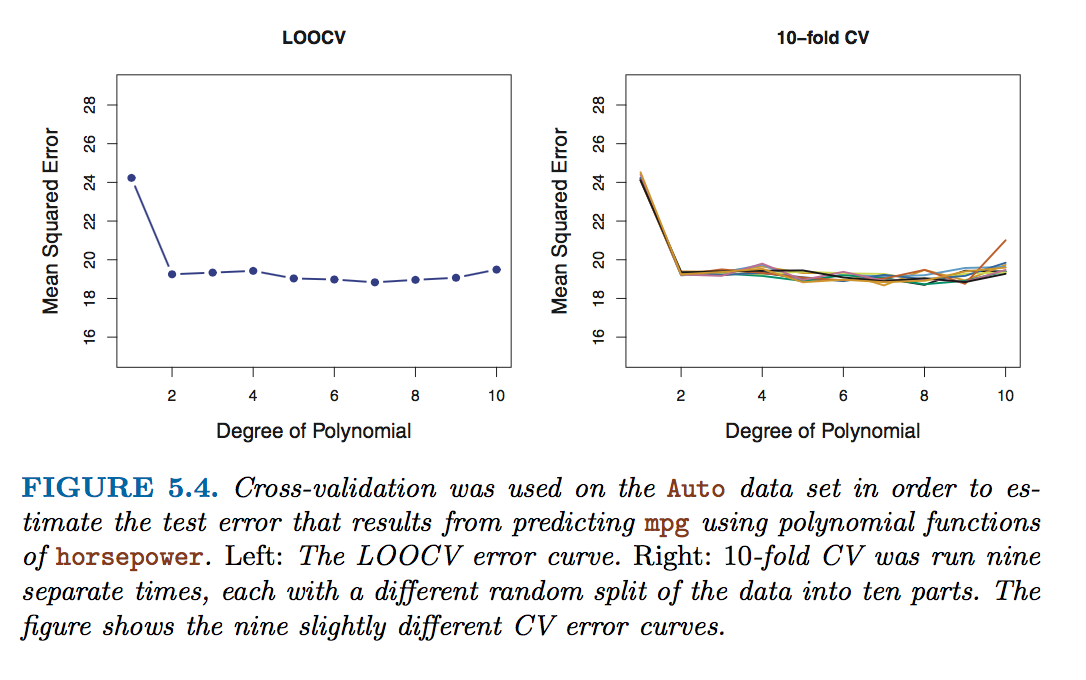
\includegraphics[width=4.5in]{./resources/comparison-cv}
\end{center}
\end{frame}

\begin{frame}{Cross Validation}
\begin{itemize}
\item Main advantage of cross validation is that we use all of the data in both \alert{estimation} and in \alert{validation}.
\begin{itemize}
\item For our purposes validation is mostly about choosing the right bandwidth or tuning parameter.
\end{itemize}
\item We have much lower variance in our estimate of the OOS mean squared error.
\begin{itemize}
\item Hopefully our bandwidth choice doesn't depend on randomness of splitting sample.
\end{itemize}
\end{itemize}
\end{frame}



\begin{frame}{Test Data}
\begin{itemize}
\item In Statistics/Machine learning there is a tradition to withhold 10\% of the data as \alert{Test Data}.
\item This is \alert{completely new data} that was not used in the CV procedure.
\item The idea is to report the results using this test data because it most accurately simulates true OOS performance.
\item We don't do much of this in economics.\\
 (Should we do more?)
\end{itemize}
\end{frame}





\end{document}